% NetSci 2018

% \documentclass[conference]{IEEEtran}

\documentclass[conference]{IEEEtran}

\usepackage{amsmath}
\usepackage{amssymb}
\usepackage{blindtext}
\usepackage{booktabs}
\usepackage{caption}
\usepackage{graphicx}
\usepackage[utf8]{inputenc}
\usepackage{multirow}
\usepackage[group-separator={,}]{siunitx}
\usepackage[x11names, rgb, dvipsnames]{xcolor}
\usepackage{xfrac}
% \usepackage[perpage]{footmisc}
% \usepackage{microtype}
\usepackage[capitalize, nameinlink, noabbrev]{cleveref}
\usepackage{subcaption}

% \usepackage{tikz}
% \usetikzlibrary{shapes}
% \usetikzlibrary{arrows}

% \bibliographystyle{alpha}
% \bibliographystyle{plain}
\bibliographystyle{unsrt}

\DeclareMathOperator{\ypred}{y_{pred}}
\DeclareMathOperator{\ytrue}{y_{true}}

\DeclareMathOperator{\rank}{rank}
\DeclareMathOperator{\cov}{cov}

\DeclareMathOperator{\TP}{TP}
\DeclareMathOperator{\TN}{TN}
\DeclareMathOperator{\FP}{FP}
\DeclareMathOperator{\FN}{FN}
\DeclareMathOperator{\FPR}{FPR}
\DeclareMathOperator{\AUC}{AUC}
\DeclareMathOperator{\TNR}{TNR}
\DeclareMathOperator{\TNA}{TNA}
\DeclareMathOperator{\TPA}{TPA}
\DeclareMathOperator{\TPR}{TPR}

\DeclareMathOperator{\Precision}{Precision}
\DeclareMathOperator{\Recall}{Recall}
\DeclareMathOperator{\InvPrecision}{Inverse\ Precision}
\DeclareMathOperator{\InvRecall}{Inverse\ Recall}
\DeclareMathOperator{\Accuracy}{Accuracy}

\DeclareMathOperator{\calls}{calls}
\DeclareMathOperator{\etime}{time}
\DeclareMathOperator{\sms}{sms}
\DeclareMathOperator{\contacts}{contacts}

\DeclareMathOperator{\ein}{in}
\DeclareMathOperator{\out}{out}

\DeclareMathOperator{\low}{low}
\DeclareMathOperator{\high}{high}

\DeclareMathOperator{\train}{train}
\DeclareMathOperator{\test}{test}

\DeclareMathOperator{\Betainc}{\Beta_{\operatorname{inc}}}

\DeclareMathOperator{\incalls}{incalls}
\DeclareMathOperator{\outcalls}{outcalls}
\DeclareMathOperator{\insms}{insms}
\DeclareMathOperator{\outsms}{insms}
\DeclareMathOperator{\intime}{outtime}
\DeclareMathOperator{\outtime}{outtime}
\DeclareMathOperator{\incontacts}{incontacts}
\DeclareMathOperator{\outcontacts}{outcontacts}

\DeclareMathOperator{\incallslow}{incallslow}
\DeclareMathOperator{\outcallslow}{outcallslow}
\DeclareMathOperator{\insmslow}{insmslow}
\DeclareMathOperator{\outsmslow}{insmslow}
\DeclareMathOperator{\intimelow}{outtimelow}
\DeclareMathOperator{\outtimelow}{outtimelow}
\DeclareMathOperator{\incontactslow}{incontactslow}
\DeclareMathOperator{\outcontactslow}{outcontactslow}

\DeclareMathOperator{\incallshigh}{incallshigh}
\DeclareMathOperator{\outcallshigh}{outcallshigh}
\DeclareMathOperator{\insmshigh}{insmshigh}
\DeclareMathOperator{\outsmshigh}{insmshigh}
\DeclareMathOperator{\intimehigh}{outtimehigh}
\DeclareMathOperator{\outtimehigh}{outtimehigh}
\DeclareMathOperator{\incontactshigh}{incontactshigh}
\DeclareMathOperator{\outcontactshigh}{outcontactshigh}

\DeclareMathOperator{\neigh}{Neigh}

\DeclareMathOperator{\dir}{dir}
\DeclareMathOperator{\cat}{cat}

\DeclareMathOperator{\ego}{ego}

\DeclareMathOperator{\logit}{logit}

\DeclareMathOperator{\Betadist}{Beta}
\DeclareMathOperator{\Binomial}{Bin}



\newcommand{\todo}[1]{\textbf{\color{red} TODO:\@ #1}}
\newcommand{\maybe}[1]{\footnote{\color{red} #1}}

\newcommand{\NA}{---}
\newcommand{\ct}[1]{\multicolumn{1}{c}{#1}}

\newcommand{\noimage}{%
  \setlength{\fboxsep}{-\fboxrule}
  \fbox{\phantom{\rule{\columnwidth}{100pt}}}
}
\newcommand{\includegraphicsmaybe}[1]{\IfFileExists{#1}{\includegraphics[width=\columnwidth, height=.24\textheight, keepaspectratio]{#1}}{\noimage}}

\renewcommand{\thefootnote}{\fnsymbol{footnote}}
\captionsetup[table]{skip = 2ex}

% \title{Comparison of Featurization Methods and Predictors for Income Inference}

\title{Featurization Methods and Predictors for Income Inference Based on Communication Patterns}

\author{%
\IEEEauthorblockN{%
	Carlos Sarraute\IEEEauthorrefmark{1},
	Martin Fixman\IEEEauthorrefmark{2},
	Martin Minnoni\IEEEauthorrefmark{1},
	Matias Travizano\IEEEauthorrefmark{1}
}
\IEEEauthorblockA{\IEEEauthorrefmark{1}Grandata Labs, 550 15th Street, San Francisco, CA, USA}
\IEEEauthorblockA{\IEEEauthorrefmark{2}Universidad de Buenos Aires, Argentina}
\IEEEauthorblockA{Email: charles@grandata.com, martinfixman@gmail.com, \{martin, mat\}@grandata.com}
}

\begin{document}
\maketitle




%%%%%%%%%%%%%%%%%%%%

Patterns of mobile phone communication, combined with underlying social network graph and financial behavior information, can be leveraged to make inferences of users' socio-economic attributes, such as their income level. We present several methods to extract features from mobile phone usage (calls and messages), and compare combinations of supervised machine learning techniques and sets of features used as input for the inference of users' income. 

For this study, we had access to a set $P$ of anonymized Call Detail Records (CDR), composed of voice calls and text messages, from a telecommunication company in a single country for a period of 3 months. Additionally, we used a set $B$ of account balances of millions of clients of one bank for a period of 6 months in the same country. 
The data of each client $b \in B$ contains the phone number anonymized with the same cryptographic function as the telco dataset, along with the average income of this person over 6 months.

We represent the network as a directed graph $G = \left< V, E \right>$, where nodes $V$ represent users and edges $E$ represent their communications. When we analyze the communications between bank clients, we observe a strong homophily in the graph with respect to the users' income, as shown in Fig.~\ref{homophily_heatmap}. This homophily is tied to the social stratification between populations of different purchasing power.

\begin{figure}[h]
\begin{center}
{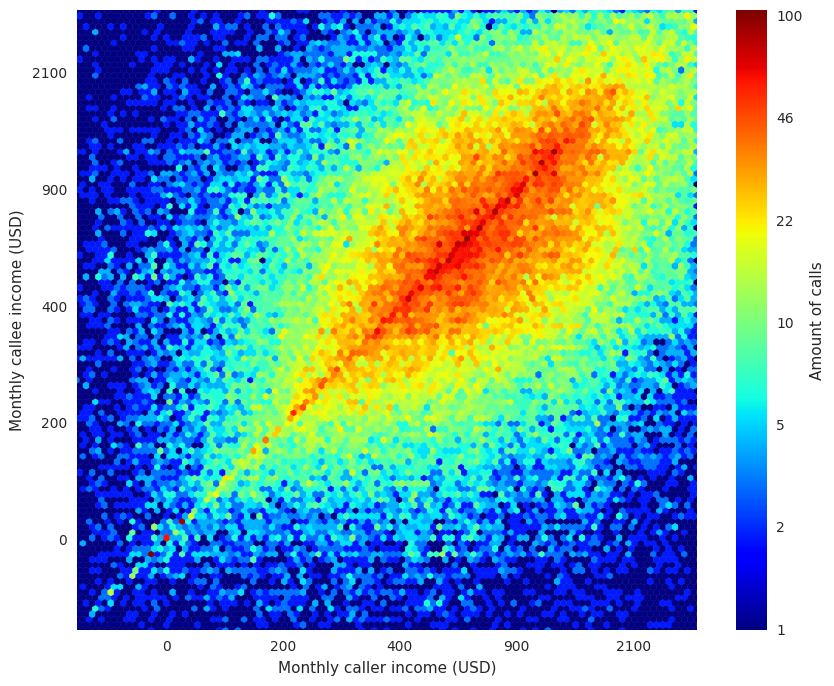
\includegraphics[width=\columnwidth]
{figures/Homophily_income_origin_target_usd.png}
}
\caption{Heatmap showing the number of calls between users, according to their monthly income. There is a higher probability that caller and callee have a similar income level.}
\label{homophily_heatmap}
\end{center}
\end{figure}




For the classification task, we divide the ground truth $T \subseteq V$ of the data in two  groups of equal size: \emph{High Income} and \emph{Low Income}.
Each edge $e \in E$ contains the information: total number of calls; total time (in seconds) of all the calls; and total number of messages exchanged.

We analyze several ways of transforming data from the graph $G$ into individual features.
First, we aggregate the number of calls, total time and SMS for every node, separated by whether these features are incoming or outgoing.
Then we extend this featurization to nodes in the \emph{ego network of order $n$} of a node $v$, which is the subgraph composed of all the nodes which are at distance at most $n$ from $v$.
In this way we are able to obtain \emph{user data of order $n$}, for $n = 1, 2, 3$.
For our experimental setting, we consider the set of nodes which have at least one neighbor with income information, called the \emph{Inner Graph} $F$.
In $F$ each edge feature is further separated in two features, depending on the category of the other endpoint (high or low income), obtaining a total of 72 features per node.

The inferences based on features aggregated by node were performed using \emph{Logistic Regression} and \emph{Random Forest} classifiers.
Finally, we compare the results with the \emph{Bayesian Method} presented in~\cite{fixmanasonam2016}, which only uses the amount of \emph{High Income} and \emph{Low Income} users in the ego network. 

Our experiments show that the Bayesian Method obtains an AUC = 0.746, which provides a better prediction than either the Logistic Regression (AUC = 0.693) or Random Forest (AUC = 0.714) machine learning methods using the most comprehensive set of features. 
From these results, we reach the conclusion that, in this particular case, \emph{smaller is better}. The {machine learning} methods which use many features, despite these features being informative,  are less effective at predicting the socio-economic level than the Bayesian Method which only uses two simple communication graph features.


\bibliography{../Tesis/bibliography/sna}{}

\end{document}
